\section{The SkelCL Library}
\label{section:skelcl-library}
In this section we discuss the \SkelCL Library, our implementation of the \SkelCL programming model.
It provides a \Cpp~\API that implements the features of the \SkelCL programming model, and thus liberates the application developer from writing low-level code.
In addition, the library provides some commonly used utility functions, \eg, for program initialization.
The \SkelCL Library is open source software and available at: \url{http://skelcl.uni-muenster.de}.

We start our discussion with an example showing how to use the \SkelCL library.
We describe the syntax used to represent the \SkelCL programming model introduced in the previous section.
This will include a discussion of \Cpp techniques used to implement the library.
We then shift the focus to the implementations of the memory management, algorithmic skeletons, and distributions.

\subsection{Programming with the SkelCL Library}

\autoref{lst:skelcl:dotproduct} shows the implementation of the dot product computation, discussed in the previous section, in \SkelCL.
After inlcuding the appropiate \SkelCL headers (lines~\autoref{lst:skelcl:dotproduct:inc:start}--\autoref{lst:skelcl:dotproduct:inc:end}) the \SkelCL library can be initialized as seen in line~\autoref{lst:skelcl:dotproduct:init}.
This will perform the initializations required by \OpenCL.
It is possible to provide arguments to the \code{init} function to specify which \OpenCL devices should be used by \SkelCL.
The dot product is specified using the \zip and \reduce skeletons.
The skeletons are created using \code{zip} (line~\autoref{lst:skelcl:dotproduct:zip}) and \code{reduce} (line~\autoref{lst:skelcl:dotproduct:reduce}) functions which expect the customizing functions of the skeletons as argument.
Here we use \Cpp lambda expressions (lines~\autoref{lst:skelcl:dotproduct:zip:lambda} and \autoref{lst:skelcl:dotproduct:reduce:lambda}) to specify the customizing functions.
We create the two input \code{Vector}s from C style pointers in this example (lines~\autoref{lst:skelcl:dotproduct:vecA} and \autoref{lst:skelcl:dotproduct:vecB}).
In line~\autoref{lst:skelcl:dotproduct:apply} we perform the computation by applying the customized skeletons to the data, before we finally return the computed result in line~\autoref{lst:skelcl:dotproduct:return}.

\begin{lstlisting}[%                                                             
caption={Implementation of the dot product computation in SkelCL},%
float=t,%
numbers=left,%
label={lst:skelcl:dotproduct}]
#include <SkelCL/SkelCL.h>$\label{lst:skelcl:dotproduct:inc:start}$
#include <SkelCL/Zip.h>
#include <SkelCL/Reduce.h>
#include <SkelCL/Vector.h>$\label{lst:skelcl:dotproduct:inc:end}$

float dotProduct(const float* a, const float* b, int n) {

  skelcl::init();$\label{lst:skelcl:dotproduct:init}$

  auto mult = skelcl::zip( $\label{lst:skelcl:dotproduct:zip}$
      [](float x, float y) { return x*y; } );$\label{lst:skelcl:dotproduct:zip:lambda}$
  auto sum  = skelcl::reduce($\label{lst:skelcl:dotproduct:reduce}$
      [](float x, float y) { return x+y; }, 0 );$\label{lst:skelcl:dotproduct:reduce:lambda}$

  skelcl::Vector<float> A(a, a+n);$\label{lst:skelcl:dotproduct:vecA}$
  skelcl::Vector<float> B(b, b+n);$\label{lst:skelcl:dotproduct:vecB}$

  skelcl::Vector<float> C = sum( mult(A, B) );$\label{lst:skelcl:dotproduct:apply}$

  return C.front();$\label{lst:skelcl:dotproduct:return}$
}
\end{lstlisting}

\autoref{lst:skelcl:dotproduct} shows that the \SkelCL library integrates nicely with \Cpp.
The interface of the \code{Vector} class looks familiar to \Cpp programmers and the usage of modern \Cpp features like lambda expressions and type deduction (\code{auto}) simplify the programming:
functions can be defined directly inline and type information can be omitted.

We will discuss how our implementation enables this level of integration in the next section.


\subsection{Syntax and Integration with \Cpp}
\label{section:skelcl-library:syntax}

The \SkelCL library is built on top of \OpenCL.
This has benefits as well as introduces technical challenges.
One of the technical challenges is, that \OpenCL requires the kernel to be specified as a string in the host program.
While this enables portability across different hardware architectures, it also introduces a burden on the application developer as strongly typing cannot be guarantied statically when the host program is compiled.
For the implementation of \SkelCL we choose to address this issue using a two-step implementation.
In the first step a custom compiler transforms the source code as seen in \autoref{lst:skelcl:dotproduct} to a representation where the kernel computations are represented as strings as required by \OpenCL.
In the second step the transformed program is compiled with a traditional \Cpp compiler to produce the final executable.

This allows us to free the user from writing strings in their application code and maintain the usual type safety guarantees from \Cpp at compile time.
Furthermore, we implemented type inference capabilities in our source-to-source compiler to free the application developer from specifying type information explicitly.
Our two-step design also allows application developers to compile their application code into a form which then can be deployed on systems where it might be difficult to install a custom compiler.

In the next paragraph we will start the discussion of our source-to-source compiler tool.
We will discuss how our custom compiler, together with our template-based implementation helps to maintain strong type safety at compile time.
Finally, we will look at issues regarding the integration with \Cpp like sharing code between host and device code.

\paragraph{The custom SkelCL compiler: \code{skelclc}}
To allow a deep integration of \SkelCL code with \Cpp we implemented a custom compiler: \code{skelclc}.
We leverage the LLVM infrastructure~\cite{Lattner2004} for building the compiler.
LLVM and the related Clang project offer well defined application programming interfaces for writing C and \Cpp related compiler tools.
In particular the \emph{LibTooling} API allows for writing tools which search for particular patterns in the abstract syntax tree (AST) which is representing the source code and perform actions on the found code fragments.
The \code{skelclc} tool does exactly this.
For example the tool searches for expressions like this:
\begin{lstlisting}[numbers=none,label={lst:skelclc:before},caption={Code snippet before transformation.}]
auto mult = skelcl::zip([](float x, float y){return x*y;});
\end{lstlisting}
and replaces it with:
\begin{lstlisting}[numbers=none,label={lst:skelclc:after},caption={Code snippet after transformation.}]
auto mult = skelcl::Zip<Container<float>(Container<float>,
                                         Container<float>)>(
              skelcl::Source("float func(float x, float y)"\
                             " { return x*y; }"), "func");
\end{lstlisting}

In this example the \code{zip} function has been transformed into an call of the constructor of the \code{Zip} class and the lambda expression has been transformed into a string.
Furthermore, type information have been added to the templated \code{Zip} class, which have been inferred from the lambda expression.

The user is free to write the expression in \autoref{lst:skelclc:after} explicitly, but it is arguably more convenient to write the expression in \autoref{lst:skelclc:before} and let our custom compiler perform the transformation automatically.

For every skeleton available in \SkelCL there exist a function like \code{zip} which is transformed by \code{skelclc} to a call of the constructor of the corresponding skeleton class.

\paragraph{Maintaining type safety}
Each skeleton in \SkelCL is represented by a templated class, as seen in \autoref{lst:skelclc:after}.
The template arguments of the skeleton define the types which can be used when executing the skeleton.
When executing a skeleton \code{skeleton<T(U)>} an object of type \code{U} has to be provided to receive an object of type \code{T}.
In this respect skeletons behave exactly like functions in \Cpp which can be represented using the \code{std::function<T(U)>} template class.
Skeletons taking more then one argument (like the \code{zip} skeleton) are represented as \code{skeleton<T(U, V)>} using the \emph{variadic template} feature of \Cpp.

When performing the transformations \code{skelclc} infers the types used as template arguments of the skeleton class.
To do so, it determines the types of the lambda expression arguments and its result type.
For \autoref{lst:skelclc:before} this is: \code{float} and \code{float} as argument types and \code{float} as result type.
The result type is inferred following standard \Cpp rules.
Based on this types the template arguments of the skeleton are constructed.

The skeletons \map, \zip, and \stencil can operate on either \code{Vector} or \code{Matrix}.
For these skeletons it must be possible to execute the skeleton with either a \code{Vector} or a \code{Matrix}.
To allow this, the templated class \code{Container} was introduced.
Using the template specialization mechanism, the mentioned skeletons have a special implementation when \code{Container} is used as a template argument.
In this case the classes provide two distinct overloaded member functions for execution using \code{Vector} or \code{Matrix}.

Type safety is guarantied, as the templated skeleton classes can only be executed with a container of compatible type and the type inference ensures that the user function has exactly the same type as the template argument of the skeleton class.
Therefore, applying the user function to the input data is always a type safe operation.

Because skeletons are strongly types the composition of skeletons is type safe as well, \ie, in \autoref{lst:skelcl:dotproduct} type safety between the two skeletons is guaranteed.
If the result type of \code{zip} would not match the input type of \code{reduce} a compile time error would occur.

\todo{Continue here ...}
\paragraph{Integration with \Cpp}
% shared types, shared functions, lambda captures


\subsection{Memory Management Implementation}
\label{section:skelcl-library:memory-management}
In the \SkelCL programming model the user managed its memory using \emph{container data types}.
The two container data types -- vector and matrix -- are implemented as template classes in the \SkelCL Library.
This generic implementation allows for storing data items of any primitive C/\Cpp data type (\eg, \code{int}), as well as user-defined data structures (\code{struct}s).

\paragraph{The SkelCL Vector}
The \SkelCL vector replicates the interface of the vector from the Standard Template Library (\STL), \ie, it can be used as a drop-in replacement of the standard vector.
Internally, a vector comprises pointers to corresponding areas of main memory (accessible by the host) and device memory.
The vector holds one pointer for the host and one pointer for each device available.
Memory on the devices is allocated automatically, according to the distribution of the vector:
while for a single distributed vector only memory on a single device is allocated, for a vector distributed with the copy, block, or overlap distribution memory on all devices is allocated.
The selected distribution obviously also influences how big the buffers allocated on the devices are.

Before the execution of a skeleton, the input vector's implementation ensures that all of its data is available on the devices.
This might result in implicit data transfers from the host memory to device memory.
The data of the output vector is not copied back to the host memory but rather resides in the device memory.
Before every data transfer, the vector implementation checks whether the data transfer is necessary;
only then the data is actually transferred.
Hence, if an output vector is used as the input to another skeleton, no further data transfer is performed.
This \emph{lazy copying} defers data transfers as long as possible or avoids them completely and, thus, minimizes the costly data transfers between host and device.
While all data transfers are performed implicitly by \SkelCL we understand that advanced application developers want fine grained control over the data transfers between host and devices.
For that purpose \SkelCL offers a set of \APIs developers can use to explicitly initiate and control the data transfer to and from the devices.

%In a SkelCL program, a vector object can be created and filled with data like this:
%\vspace{.5em}
%\centerline{\lstinline!Vector<int> vec(size);!}
%\centerline{\lstinline!for (int i = 0; i < vec.size(); ++i) \{ vec[i] = i; \}!}
%\vspace{.5em}

\paragraph{The SkelCL Matrix}
The \SkelCL matrix offers an easy to use interface similar to the interface of the vector.
Data is stored in row-major order and iterators are provided to iterate first over rows and then inside of a single row to access a particular element.
For the copy, block, and overlap distribution the matrix is divided across rows.
A single row is never split across multiple devices, which simplifies the memory management.
Besides offering an interface to access elements on the host, the matrix also offers an interface for accessing elements on the device by using two-dimensional indices.
This frees the application developer from performing cumbersome index calculations manually.

\subsection{Algorithmic Skeletons Implementation}
\label{section:skelcl-library:skeletons}


\subsection{Distribution Implementation}
\label{section:skelcl-library:distribution}

% TODO: ...


%\begin{itemize}
%  \item 
%    In a SkelCL program, a map skeleton is created as an object for a unary function $f$, e.\,g. negation, like this:
%
%    \vspace{.5em}
%    \centerline{\lstinline!Map<float(float)> neg("float func(float x) \{ return -x;\}");!}
%    \vspace{.5em}
%
%    This map object can then be called as a function with a vector as argument:
%
%    \vspace{.5em}
%    \centerline{\lstinline!resultVector = neg( inputVector );!}
%    \vspace{.5em}
%  \item The zip skeleton operates on two vectors $cl$ and $cr$, applying a binary customizing operator $\oplus$ pairwise:
%    \vspace{-.5em}
%    \[ zip\ (\oplus)\ [cl_1, cl_2, \dots, cl_n]\ [cr_1, cr_2, \dots, cr_n] = [cl_1\oplus cr_1, cl_2\oplus cr_2, \dots, cl_n\oplus cr_n] \]
%
%    \vspace{-.5em}
%    In SkelCL, a zip skeleton object for adding two vectors is created like as:
%
%    \vspace{.5em}
%    \centerline{\lstinline!Zip<float(float, float)> add("float func(float x,float y) \{return x+y;\}");!}
%    \vspace{.5em}
%
%    and can then be called as a function with a pair of vectors as arguments:
%
%    \vspace{.5em}
%    \centerline{\lstinline!resultVector = add( leftVector, rightVector );!}
%    \vspace{.5em}
%    
%  \item The reduce skeleton computes a scalar value from a vector using a binary associative operator $\oplus$, i.\,e.
%    \vspace{-.5em}
%    \[ red\ (\oplus)\ [v_1, v_2, \dots, v_n] = v_1 \oplus v_2 \oplus \dots \oplus v_n \]
%
%    \vspace{-.5em}
%    For example, to sum up all elements of a vector, the reduce skeleton is created with addition as customizing function, and called as follows:
%
%    \vspace{.5em}
%    \centerline{\lstinline!Reduce<float(float)> sumUp("float func(float x,float y) \{ return x+y;\}");!}
%    \vspace{.5em}
%    \centerline{\lstinline! result = sumUp( inputVector );!}
%    \vspace{.5em}
%
% 
%  \item The scan skeleton (a.\,k.\,a. prefix-sum) yields an output vector with each element obtained by applying a binary associative operator $\oplus$ to the elements of the input vector up to the current element's index, i.\,e.
%    \vspace{-.5em}
%    \[ scan\ (\oplus)\ [v_1, v_2, \dots, v_n] = [v_1, v_1\oplus v_2, \dots, v_1\oplus v_2\oplus \dots \oplus v_n] \]
%
%    \vspace{-.5em}
%    The prefix sums customized with addition is specified and called in SkelCL as follows:
%
%    \vspace{.5em}
%    \centerline{\lstinline!Scan<float(float)> prefixSum("float func(float x,float y) \{return x+y;\}");!}
%    \vspace{.5em}
%    \centerline{\lstinline! result = prefixSum( inputVector );!}
%    \vspace{.5em}
%
%\end{itemize}


% HIPS
The parallelization approach for \texttt{Reduce} depends on whether the binary operator is commutative and/or associative.
SkelCL requires the operator to be associative, such that it can be applied to arbitrarily sized subranges of the input vector in parallel.
The final result is obtained by recursively combining the intermediate results for the subranges.
To improve the performance, SkelCL saves the intermediate results in the device's fast local memory.


% additional arguments
For flexibility, \SkelCL skeletons can accept additional arguments if the customizing function works not only on a skeleton's input containers, but needs access to additional data~\cite{StKG-11};
containers passed as additional arguments to a skeleton are automatically transfered to the GPUs.

% opencl interop
SkelCL can also be used in combination with existing OpenCL codes, as SkelCL is designed as an extension of OpenCL, rather than a replacement for it.

% front end compiler

% skeleton implementation
In OpenCL, kernels are compiled at runtime of the host program in order to be executable on different GPUs.
Therefore, in the SkelCL library implementation, the customizing functions are provided as strings to their skeletons.
SkelCL implementation merges the customizing function with the pre-implemented skeleton-specific program code to build a valid OpenCL kernel automatically.
The generated kernel fetches one or more data items from its input containers (vectors or matrices), passes them to the customizing function, and yields the function's result, e.\,g., by writing it to the output container.
Rather than working with pointers to GPU memory (like kernels do), customizing functions in SkelCL take a single data item as input and return a single result.
The SkelCL implementation of the vector container resembles the interface of the vector from the C++ Standard Template Library (STL), i.\,e., it can be used as a replacement for the standard vector.
Internally, the containers manage pointers to the corresponding areas of the main memory (accessible by the CPU) and GPU memory.
For possible optimizations of the kernel's source code, we rely on the optimization capabilities of the OpenCL compiler.

% data transfers
In some situations, our SkelCL implementation can optimize data transfers:
\eg, after executing a skeleton, the output data remains in the GPU memory;
this has the advantage that if the output container is used as the input to another skeleton, no data transfer has to be performed.
Such \emph{lazy copying} implemented in SkelCL minimizes costly data transfers between the CPU and GPUs.



%% MapOverlap / Stencil implementation

% In the actual source code, the application developer provides the function $f$ which receives a pointer to the element in the middle, $m_{in}[i,j]$.
% Listing~\ref{lst:mapoverlap01} shows a simple example of computing the sum of all direct neighboring values using the MapOverlap skeleton.
% To access the elements of the input matrix $m_{in}$, function \texttt{get} is used, as provided by SkelCL.
% All indices are specified relative to the middle element $m_{in}[i,j]$, therefore, for accessing this element the function call \texttt{get(m\_in, 0, 0)} is used.

% The application developer must ensure that only elements in the range specified by the second argument $d$ of the MapOverlap skeleton, are accessed.
% In Listing~\ref{lst:mapoverlap01}, range is specified as $d=1$, therefore, only direct neighboring elements are accessed.
% To enforce this property, boundary checks are performed at runtime by the \texttt{get} function.
% In future work, we plan to avoid boundary checks at runtime by statically proving that all memory accesses are in bounds, as it is the case in the shown example.


% \begin{lstlisting}[%
% caption={MapOverlap skeleton computing the sum of all direct neightbors for every element in a matrix},%
% float=tbp,%
% label={lst:mapoverlap01}]
% MapOverlap<float(float)> m("float func(float* m_in){
%      float sum = 0.0f;
%      for (int i = -1; i < 1; ++i)
%        for (int j = -1; j < 1; ++i)
%          sum += get(m_in, i, j);
%      return sum;
%    }", 1, SCL_NEUTRAL, 0.0f);
% \end{lstlisting}

% Listing~\ref{lst:raw_opencl01} shows how the same simple calculation can be performed in standard OpenCL.
% While the amount of lines of code increases by a factor of 2, the complexity of each single line also increases, as follows.
% Besides a pointer to the output memory, the width of the matrix has to be provided as parameter.
% The correct index has to be calculated for every memory access using an offset and the width of the matrix.
% Therefore, knowledge about how the two-dimensional matrix is stored in one-dimensional memory is required.
% In addition, manual boundary checks have to be performed to avoid faulty memory accesses.\bigskip

% \begin{lstlisting}[%
% caption={An OpenCL kernel performing the same calculation as the MapOverlap skeleton shown in Listing~\ref{lst:mapoverlap01}.\bigskip},%
% label={lst:raw_opencl01}]
% __kernel void sum_up(__global float* m_in,
%                      __global float* m_out,
%                      int width, int height) {
%   int i_off = get_global_id(0); int j_off = get_global_id(1);
%   float sum = 0.0f;
%   for (int i = i_off - 1; i < i_off + 1; ++i)
%     for (int j = j_off - 1; j < j_off + 1; ++j) {
%       // perform boundary checks
%       if ( i < 0 || i > width || j < 0 || j > height )
%         continue;
%       sum += m_in[ j * width + i ];     }
%   m_out[ j_off * width + i_off ] = sum; }
% \end{lstlisting}

% SkelCL avoids all these low-level details.
% Neither additional parameter, nor index calculations or manual boundary checks are necessary.
% In SkelCL, the application developer only provides the source code implementing the steps required by the algorithm.


% In the actual source code, the application developer provides the function $f$ which receives a pointer to the element in the middle, $m_{in}[i,j]$.

% \begin{lstlisting}[%
% caption={MapOverlap skeleton computing the sum of all direct neightbors for every element in a matrix},%
% float=bp,%
% label={lst:mapoverlap01}]
% MapOverlap<float(float)> m("float func(float* m_in){
% float sum = 0.0f;
% for (int i = -1; i < 1; ++i)
%   for (int j = -1; j < 1; ++i)
%     sum += get(m_in, i, j); return sum;
% }", 1, SCL_NEUTRAL, 0.0f);
% \end{lstlisting}


% Listing~\ref{lst:mapoverlap01} shows a simple example of computing the sum of all direct neighboring values using the MapOverlap skeleton.
% To access the elements of the input matrix $m_{in}$, function \texttt{get} is provided by SkelCL.
% All indices are specified relative to the middle element $m_{in}[i,j]$; therefore, for accessing this element the function call \texttt{get(m\_in, 0, 0)} is used.
% The application developer must ensure that only elements in the range specified by the second argument $d$ of the MapOverlap skeleton, are accessed.
% In Listing~\ref{lst:mapoverlap01}, range is specified as $d=1$, therefore, only direct neighboring elements are accessed.
% To enforce this property, boundary checks are performed at runtime by the \texttt{get} function.
% In future work, we plan to avoid boundary checks at runtime by statically proving that all memory accesses are in bounds, as it is the case in the shown example.

% \begin{lstlisting}[%
% caption={An OpenCL kernel performing the same calculation as the MapOverlap skeleton shown in Listing~\ref{lst:mapoverlap01}.},%
% float=tbp,%
% label={lst:raw_opencl01}]
% __kernel void sum_up(__global float* m_in,
%                      __global float* m_out,
%                      int width, int height) {
%   int i_off = get_global_id(0); 
%   int j_off = get_global_id(1);
%   float sum = 0.0f;
%   for (int i = i_off - 1; i < i_off + 1; ++i)
%     for (int j = j_off - 1; j < j_off + 1; ++j) {
%       // perform boundary checks
%       if ( i < 0 || i > width || j < 0 || j > height )
%         continue;
%       sum += m_in[ j * width + i ];     }
%   m_out[ j_off * width + i_off ] = sum; }
% \end{lstlisting}


% Listing~\ref{lst:raw_opencl01} shows how the same simple calculation can be performed in standard OpenCL.
% While the amount of lines of code increases by a factor of 2, the complexity of each single line also increases:
% 1) Besides a pointer to the output memory, the width of the matrix has to be provided as parameter; 2) the correct index has to be calculated for every memory access using an offset and the width of the matrix, i.\,e.
% knowledge about how the two-dimensional matrix is stored in one-dimensional memory is required.
% 3) In addition, manual boundary checks have to be performed to avoid faulty memory accesses. 

% SkelCL avoids all these low-level details.
% Neither additional parameter, nor index calculations or manual boundary checks are necessary.



% \from{HiStencils}
% Listing~\ref{lst:mapoverlap01} shows the implementation of the Sobel edge detection using the \emph{MapOverlap} skeleton.
% The MapOverlap skeleton applies a given function $func$ (defined in lines 2--6) to each element of an input matrix $in_{img}$ while taking the neighboring elements within the range $[-d, +d]$ in each dimension into account.
% Here, $d$ is the second parameter (line 7) and two additional parameters define how the skeleton handles out-of-bound memory accesses (line 8).
% A helper function (\code{get}) is used to easily access the neighboring elements.
% The indexes are specified relative to the current element, e.\,g. to access the element on the left the function call \code{get(in, -1, 0)} is used.

% Special handling is necessary when accessing elements out of the boundaries of the matrix, e.g., when the item in the top-left corner of the matrix accesses elements above and left of it.
% The MapOverlap skeleton can be configured to handle such out-of-bound memory accesses in two possible ways:
% 1) a specified neutral value is returned;
% 2) the nearest valid value inside the matrix is returned.
% In Listing~\ref{lst:mapoverlap01}, the first option is chosen and $0$ is provided as neutral value.

% \begin{lstlisting}[%
% caption={Implementation of Sobel edge detection using the MapOverlap skeleton},%
% float=tbp,%
% label={lst:mapoverlap01}]
% MapOverlap<char(char)> sobel(
%  "char func(const char* in_img) {
%     char ul = get(in_img, -1, -1);
%     ...
%     char lr = get(in_img, +1, +1);
%     return computeSobel(ul,..., lr);}",
%  1, Padding::NEUTRAL, 0);

% output = sobel(input);
% \end{lstlisting}

% Simple stencil computations with a regular stencil shape can easily be expressed using the MapOverlap skeleton.
% For more complex stencil computations, e.\,g. iterative stencils, we introduce the more advanced \emph{Stencil} skeleton.

% \paragraph{The MapOverlap Skeleton}

% Listing~\ref{lst:stencil01} shows the implementation of an iterative stencil application simulating heat transfer.
% This application simulates heat spreading from one location and flowing throughout a two-dimensional simulation space.
% \begin{lstlisting}[%
% caption={Implementation of heat simulation using the Stencil skeleton},%
% float=tbp,%
% label={lst:stencil01}]
% Stencil<char(char)> heatSim(
%  "char func(const char* in) {
%     char lt = get(in, -1, -1);
%     char lm = get(in, -1,  0);
%     char lb = get(in, -1, +1);
%     return computeHeat(lt, lm, lb); }",
%  StencilShape(1, 0, 1, 1),
%  Padding::NEUTRAL, 255);

% output = heatSim(100, input);
% \end{lstlisting}


% The application developer specifies the function (line 2--6) describing the computation and, therefore, the stencil shape, as well as the stencil shape's extents (line 7) and the out-of-bound handling (line 8).
% The stencil shape's extents are specified using four values for each of the directions:
% up, right, down, left.
% In the example in Listing~\ref{lst:stencil01}, the heat flows from left to right, therefore, no accesses to elements to the right are necessary and the stencil space's extents are specified accordingly (note the $0$ in line 7 representing the extent to the right).
% Figure~\ref{fig:stencilShape} illustrates this situation: the dark gray element is updated by using the values from the left.
% The specified stencil shape's extent is highlighted in light gray.
% In our current implementation, the user has to explicitly specify the stencil shape's extents, which is necessary for performing the out-of-bound handling on the GPU.
% In future work, we plan to automatically infer the stencil shape's extents
% from the customizing function using source code analysis in order to free the user from specifying this information explicitly.
% \begin{figure}
%   \begin{centering}
%     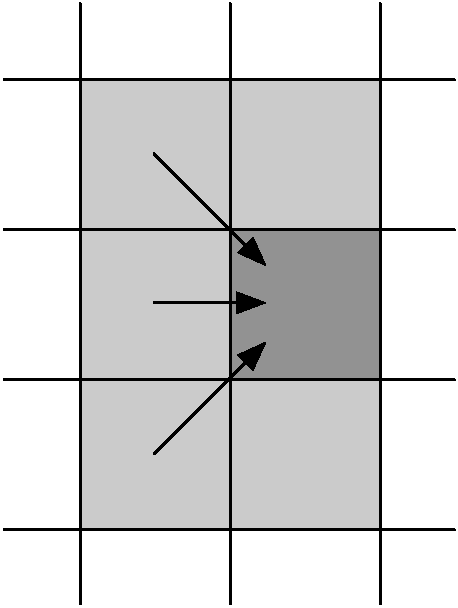
\includegraphics[width=.18\textwidth]{HiStencils/heat_transfer}
%     \caption{Stencil shape for heat transfer simulation}
%     \label{fig:stencilShape}
%     \vspace{-.5em}
%   \end{centering}
% \end{figure}

% Many stencil applications apply a stencil multiple times for a fixed number of iterations, or until a certain condition is met.
% For example, to iterate the heat transfer simulation for one hundred steps, we specify the number of iterations to perform when executing the skeleton (line 10).
% In the future, we plan to allow the user to specify a custom function which checks a condition to stop the iterations.

% The MapOverlap skeleton can be configured to handle out-of-bounds accesses by returning the nearest valid value of the input matrix.
% Another distinction can be made regarding iterations and sequences of stencil operations:
% using elements of the \textbf{initial}, user-provided input matrix or using elements of the \textbf{current} step's input matrix, which already was updated during earlier stencil operations.
% The Stencil skeleton can be configured to handle out-of-bounds accesses in both ways, thus offering three possible ways, including the neutral value. 
% For each of them, there is an own kernel function, loading appropriate elements into local memory. 






% Simple stencil computations with a regular stencil shape can easily be expressed using the \mapOverlap skeleton.
% For more complex stencil computations, \eg iterative stencil computations, we introduce the more advanced \stencil skeleton.





% Real-world applications often perform multiple stencil operations in sequence.
% Let us consider the popular \emph{Canny algorithm} which is used for detecting edges in images.
% For the sake of simplicity we consider a simplified version, which applies the following stencil operations in a sequence:
% 1), a noise reduction operation is applied, e.g., a Gaussian filter;
% 2), an edge detection operator like the Sobel filter is applied;
% 3), the so-called non-maximum suppression is performed, where all pixels in the image are colored black except pixels being a local maximum;
% 4), a threshold operation is applied to produce the final result.
% A more complex version of the algorithm performs the edge tracking by hysteresis, as an additional step.
% This results in detecting some weaker edges, but even without this additional step the algorithm usually achieves good results.

% In SkelCL, each single step of the Canny algorithm can be expressed using the Stencil skeleton.
% The last step, threshold operation, does not need access to neighboring elements, as the user threshold function only checks the value of the current pixel.
% Therefore, this step can be expressed using SkelCL's simpler Map skeleton.
% The Stencil skeleton's implementation automatically uses the simpler Map skeleton's implementation when the user specifies a stencil shape which extents are $0$ in all directions.

% \begin{lstlisting}[%
%   caption={Structure of the Canny algorithm as implemented with a sequence of skeletons.},%
%   float=tbp,%
%   label={lst:canny01}]
% Stencil<Pixel(Pixel)> gauss(...);
% Stencil<Pixel(Pixel)> sobel(...);
% Stencil<Pixel(Pixel)> nms(...);
% Stencil<Pixel(Pixel)> threshold(...);

% StencilSequence<Pixel(Pixel)> canny(
%   gauss, sobel, nms, threshold);

% output = canny(1, input);
% \end{lstlisting}

% To implement the Canny algorithm in SkelCL, the single steps can be combined as shown in Listing~\ref{lst:canny01}.
% The individual steps are defined in lines 1--4 and then combined to a sequence of stencils in line 6 and 7.
% During execution (line 9), the stencil operation are performed in the order which is specified when creating the \emph{StencilSequence} object.

% \paragraph{Implementation}
% In order to achieve high performance, our implementations of both the MapOverlap and the Stencil skeleton use the GPU's fast local memory.
% Both implementations perform the same basic steps on the GPU:
% first, the data is loaded from the global memory into the local memory;
% then, the user-defined function is called for every data element by passing a pointer to the element's location in the local memory;
% finally, the result of the user-defined function is copied back into the global memory.

% Although both implementations perform the same basic steps, different strategies are implemented for loading the data from the global into the local memory.

% \begin{figure}
%   \begin{centering}
%     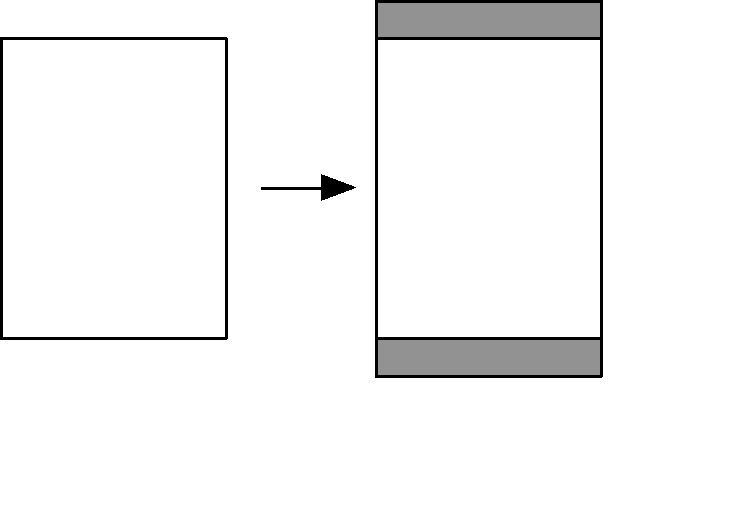
\includegraphics[width=.29\textwidth]{HiStencils/map_overlap}
%     \caption{The MapOverlap skeleton prepares a matrix by copying data on the top and bottom.}
%     \label{fig:preparation}
%     \vspace{-.5em}
%   \end{centering}
% \end{figure}

% The MapOverlap skeleton prepares the input matrix on the CPU before uploading it to the GPU:
% padding elements are appended; they are used to avoid out-of-bounds memory accesses to the top and bottom of the input matrix, as shown in Figure~\ref{fig:preparation}.
% This slightly enlarges the input matrix, but it reduces branching on the GPU due to avoiding some out-of-bound checks.
% In SkelCL a matrix is stored row-wise in memory on the CPU and GPU, therefore, it would be complex and costly to add padding elements on the left and right of the matrix.
% To avoid out-of-bound accesses for these regions, the boundary checks are performed on the GPU.

% The Stencil skeleton has to use a different strategy in order to enable the usage of different padding modes and stencil shapes when using several Stencil skeletons in a sequence.
% As an example, consider two stencil shapes in a sequence where the first shape defines a neutral element $0$ and the second defines a neutral element $1$.
% This cannot be implemented using MapOverlap's implementation strategy.
% Therefore, Stencil does not append padding elements on the CPU, but rather manages all out-of-bounds accesses on the GPU, which slightly increases branching.

% \section{Targeting Multi-GPU Systems (HiStencils)}
% \label{sec:multi_gpu}
% The implicit and automatic support of systems with multiple OpenCL devices is one of the key features of SkelCL.
% By using distributions, SkelCL completely liberates the user from error-prone and low-level explicit programming of data (re)distributions on multiple GPUs. 

% The MapOverlap skeleton uses the overlap distribution with \textit{border regions} in which the elements calculated by a neighboring device are located.
% When it comes to iteratively executing a skeleton, data has to be transferred among devices between iteration steps, in order to ensure that data for the next iteration step is up-to-date.
% As the MapOverlap skeleton does not explicitly support iterations, its implementation is not able to exchange data between devices besides a full down- and upload of the matrix.
% In addition, data exchange has to be performed after each iteration.
% We can enlarge the number of elements in the border regions and perform multiple iteration steps on each device before exchanging data.
% However, this introduces redundant computations, such that a trade-off between data exchange and redundant computations has to be found.
 
% For the Stencil skeleton, the user can specify the number of iterations between \textit{device synchronisations}, where all border regions are updated with elements from the corresponding inner border regions of the neighboring device.
% The border regions are sized by default in such a way that the specified number of iterations can be performed without leading to incorrect results.
% However, there may be cases in which a different number of iterations between device synchronizations may result in better performance.
% Therefore, Stencil offers the user the possibility to specify that number.
% Please note that the implementation of the Stencil skeleton only exchanges elements from the border region and does not perform a full down- and upload of the matrix, as the MapOverlap skeleton does.

% Figure \ref{fig:syncDevices} shows the device synchronization.
% Only the appropriate elements in the inner border region are downloaded and stored as \texttt{std::vector}s in a \texttt{std::vector}.
% Within the outer vector, the inner vectors are swapped pair-wise on the host, so that the inner border regions can be uploaded in order to replace the out-of-date border regions.

% For the first iteration after a device synchronization, there are as many work-items on the GPU active as there are total elements on the device.
% As the first and last rows of the border regions become invalid within an iteration, the corresponding work-items become inactive in the following iteration step.
% This is done by using an offset and by reducing the number of total work-items when launching the OpenCL kernel.
% The Stencil's four kernel functions (one for each out-of-bounds handling mode and one for the adapted Map skeleton) can be used for both single- and multi-GPU systems.
 
% \begin{figure}[tb]
%   \centering
%   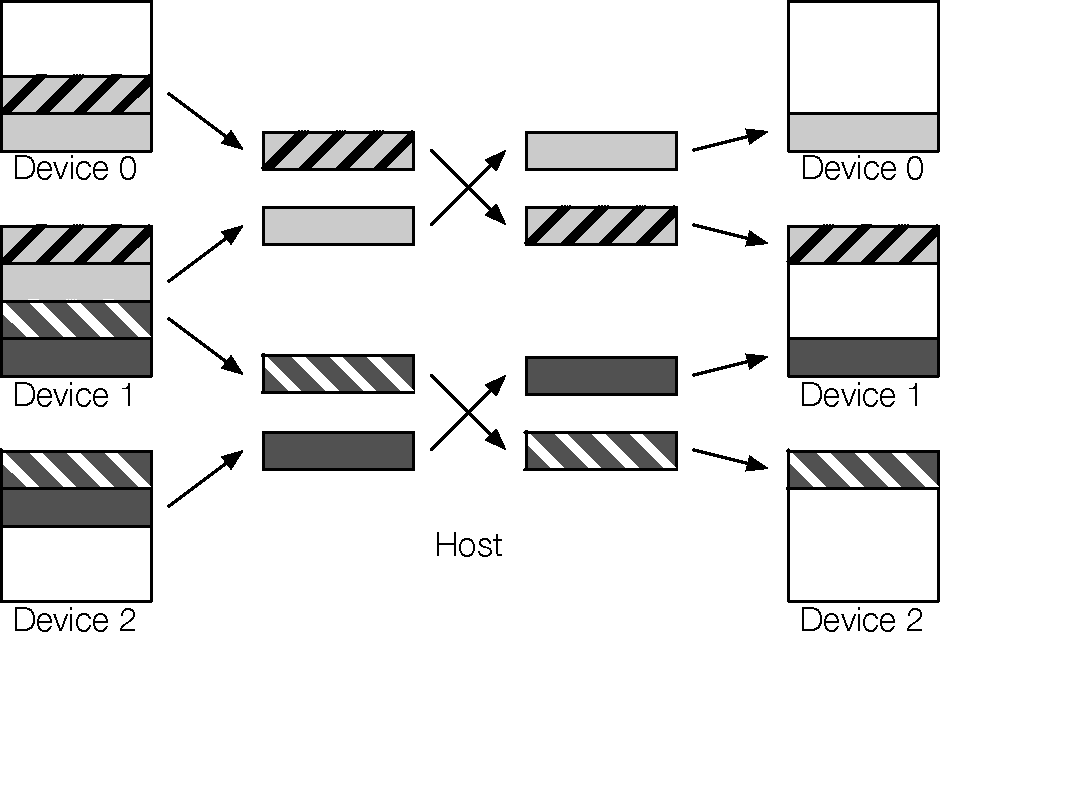
\includegraphics[width=\columnwidth]{HiStencils/data_exchange}
%   \caption{\small Device synchronization for three devices. Equally patterned and colored chunks represent the border regions and their matching inner border region. After the download of the appropriate inner border regions, they are swapped pair-wise on the host. Then the inner border regions are uploaded in order to replace the out-of-date border regions.}
%   \label{fig:syncDevices}
%   \vspace{1em}
% \end{figure} 






% allpairs impl




% \vspace{1em}
% We develop the allpairs skeleton within the skeleton library SkelCL~\cite{StKG-12}, which is built on top of OpenCL and targets modern parallel systems with multiple GPUs.
% Currently, five other skeletons are available in SkelCL: \emph{map}, \emph{zip}, \emph{reduce}, \emph{scan}, and \emph{mapOverlap}.
% Skeletons operate on container data types (in particular vectors and matrices) which alleviate the memory management of GPUs:
% data is copied automatically to and from GPUs, instead of manually performing data transfers as required in OpenCL.
% For programming multi-GPU systems, SkelCL offers the application programmer a data distribution mechanism to specify how the data of a container is distributed among the GPUs in the system.
% The container's data can either be assigned to a single GPU, be copied to all GPUs, or be partitioned in equal blocks across the GPUs, possibly with an overlap.
% If the data distribution is changed in the program, the necessary data movements are done automatically by the system~\cite{StKG-12}.

% \begin{lstlisting}[%                                                             
% caption={Matrix multiplication in SkelCL using the \emph{allpairs} skeleton.},%
% float=t,%                                                                       
% numbers=left,%
% label={lst:basic_mm}]
% skelcl::init();
% Allpairs<float(float, float)> mm(
%  "float func(float_matrix_t a, float_matrix_t b) {\
%   float c = 0.0f;\
%   for (int i = 0; i < width(a); ++i) {\
%     c += getElementFromRow(a, i) * getElementFromCol(b, i); }\
%   return c; }");
% Matrix<float> A(n, k); fill(A);
% Matrix<float> B(k, m); fill(B);
% Matrix<float> C = mm(A, B);
% \end{lstlisting}

% Listing~\ref{lst:basic_mm} shows the SkelCL program for computing matrix multiplication using the \emph{allpairs} skeleton;
% the code follows directly from the mathematical formulation (\ref{eq:mat_mult_allpairs}).
% In the first line, the SkelCL library is initialized.
% Skeletons are implemented as classes in SkelCL and customized by instantiating a new object, like in line 2.
% The \texttt{Allpairs} class is implemented as a template class specified with the data types of matrices involved in the computation (\texttt{float(float, float)}).
% This way the implementation can ensure the type correctness by checking the types of the arguments when the skeleton is executed in line 10.
% The customizing function -- specified as a string (line 3 -- 7) -- is passed to the constructor.
% Data types for matrices (\texttt{float\_matrix\_t} in line 3) are defined by the SkelCL implementation and used as arguments of helper functions for accessing elements from both matrices (line 6).
% The transpose of matrix $B$ required by the definition (\ref{eq:mat_mult_allpairs}) is implicitly performed by accessing elements from the columns of $B$ using the helper function \texttt{getElementFromCol}.
% After initializing the two input matrices (line 8 and 9), the calculation is performed in line 10.

% In our SkelCL library, skeletons are implemented by translating them into executable OpenCL code.
% Listing~\ref{lst:basic_impl} shows the OpenCL kernel which is combined with the given customizing function by the implementation of the allpairs skeleton.
% The customizing function (named \texttt{\emph{func}} in Listing~\ref{lst:basic_mm}) is renamed to match the name used in the function call in the implementation (\texttt{USER\_FUNC} in Listing~\ref{lst:basic_impl}).
% In addition, the types used in the predefined OpenCL kernel (\texttt{TYPE\_LEFT}, \texttt{TYPE\_RIGHT}, and \texttt{TYPE\_OUT} in Listing~\ref{lst:basic_impl}) are adjusted to match the actual types of the elements used in the computation (in this case, all three types are \texttt{float}).
% These modifications ensure that a valid OpenCL program performing the allpairs calculation is constructed.
% This generated OpenCL program is executed once for every element of the output matrix $C$.
% In lines 6 -- 7, the implementation prepares variables (\texttt{Am} and \texttt{Bm}) of a predefined data type (\texttt{float\_matrix\_t}) which encapsulate the matrices $A$ and $B$ and passes them to the customizing function which is called in line 9.

% \begin{lstlisting}[%                                                             
% caption={Generic OpenCL kernel used in the implementation of the allpairs skeleton.},%
% float=t,%                                                                       
% numbers=left,%
% label={lst:basic_impl}]
% __kernel void allpairs(const __global TYPE_LEFT*  A,
%                        const __global TYPE_RIGHT* B,
%                              __global TYPE_OUT*   C,
%                              int n, int d, int m) {
%   int col = get_global_id(0); int row = get_global_id(1);
%   float_matrix_t Am; Am.data = A; Am.width = d; Am.row = row;
%   float_matrix_t Bm; Bm.data = B; Bm.width = m; Bm.col = col;
%   if (row < n && col < m)
%     C[row * m + col] = USER_FUNC(Am, Bm); }
% \end{lstlisting}

% To achieve high performance, skeleton implementations must efficiently exploit the complex memory hierarchy of multi-GPU architectures.
% There are two main types of memory in OpenCL: \emph{global} and \emph{local memory}.
% The global memory is typically large but slow; the local memory is small but fast and has similar performance as caches in traditional systems, but has to be programmed manually.
% On modern GPUs, accesses to the global memory are very expensive, taking up to 800 processor cycles, as compared to only few cycles required to access the local memory~\cite{NVIDIA-12}.

% The generic implementation of the allpairs skeleton in Listing~\ref{lst:basic_impl} makes no assumption about the order in which the customizing function (\texttt{USER\_FUNC}) accesses the elements of its two input vectors.
% In this general case, we cannot assume that the two vectors fit entirely into the restricted GPU local memory.
% Therefore, we have to use only the global memory in the generic implementation.
% To improve our implementation of the allpairs skeleton, we restrict the memory access pattern of the customizing function in the next section.





% specialized allpairs

% \begin{lstlisting}[%                                                             
% caption={Matrix multiplication in SkelCL using the specialized \emph{allpairs} skeleton.},%
% float=b,%                                                                       
% numbers=left,%
% label={lst:nested_allpairs}]
% skelcl::init();
% Zip<float(float, float)> mult
%     ("float func(float x, float y) { return x*y; }");
% Reduce<float(float, float)> sum_up
%     ("float func(float x, float y) { return x+y; }");
% Allpairs<float(float, float)> mm(sum_up, mult);
% Matrix<float> A(n, d); fill(A);
% Matrix<float> B(d, m); fill(B);
% Matrix<float> C = mm(A, B);
% \end{lstlisting}

% Listing~\ref{lst:nested_allpairs} shows how the matrix multiplication can be programmed in SkelCL using the allpairs skeleton customized with zip-reduce.
% In line 1, the SkelCL library is initialized.
% In lines 2 and 3, the zip skeleton is defined using multiplication as customizing function and in lines 4 and 5, the reduce skeleton is customized with addition.
% These two customized skeletons are passed to the allpairs skeleton on its creation in line 6.
% The implementation of the allpairs skeleton then uses the two customizing functions of zip and reduce to generate the OpenCL kernel performing the allpairs computation.
% In line 9, the skeleton is executed taking two input matrices and producing the output matrix.
% Note that we create objects of the same \texttt{Allpairs} class when using the generic allpairs implementation (Listing~\ref{lst:basic_impl} line 2) and the specialized implementation (Listing~\ref{lst:nested_allpairs} line 6).
% Depending on which of the overloaded constructors is used, either the generic or the specialized implementation is created.


